% This must be in the first 5 lines to tell arXiv to use pdfLaTeX, which is strongly recommended.
\pdfoutput=1
% In particular, the hyperref package requires pdfLaTeX in order to break URLs across lines.

\documentclass[11pt]{article}

% Remove the "review" option to generate the final version.
\usepackage[review]{EMNLP2023}

% Standard package includes
\usepackage{times}
\usepackage{latexsym}

% For proper rendering and hyphenation of words containing Latin characters (including in bib files)
\usepackage[T1]{fontenc}
% For Vietnamese characters
% \usepackage[T5]{fontenc}
% See https://www.latex-project.org/help/documentation/encguide.pdf for other character sets

% This assumes your files are encoded as UTF8
\usepackage[utf8]{inputenc}

% This is not strictly necessary, and may be commented out.
% However, it will improve the layout of the manuscript,
% and will typically save some space.
\usepackage{microtype}

% This is also not strictly necessary, and may be commented out.
% However, it will improve the aesthetics of text in
% the typewriter font.
\usepackage{inconsolata}
% includegraphics
\usepackage{graphicx}
%listings
\usepackage{listings}
\usepackage{dirtytalk}

%pandas tables
\usepackage{{booktabs}}
% Commands
\newcommand{\todo}[1]{{\color{red}\colorbox{yellow}{\textbf{TODO: }}#1}}
\newcommand{\averitec}{AVeriTeC}
\newcommand{\supp}{Supported}
\newcommand{\reff}{Refuted}
\newcommand{\nei}{Not enough evidence}
\newcommand{\conf}{Conflicting evidence/Cherrypicking}
\makeatletter
\newcommand\footnoteref[1]{\protected@xdef\@thefnmark{\ref{#1}}\@footnotemark}
\makeatother

% If the title and author information does not fit in the area allocated, uncomment the following
%
%\setlength\titlebox{<dim>}
%
% and set <dim> to something 5cm or larger.

\title{AIC CTU system at \averitec{}: Re-framing automated fact-checking as a simple RAG task}

% Author information can be set in various styles:
% For several authors from the same institution:
% \author{Author 1 \and ... \and Author n \\
%         Address line \\ ... \\ Address line}
% if the names do not fit well on one line use
%         Author 1 \\ {\bf Author 2} \\ ... \\ {\bf Author n} \\
% For authors from different institutions:
% \author{Author 1 \\ Address line \\  ... \\ Address line
%         \And  ... \And
%         Author n \\ Address line \\ ... \\ Address line}
% To start a seperate ``row'' of authors use \AND, as in
% \author{Author 1 \\ Address line \\  ... \\ Address line
%         \AND
%         Author 2 \\ Address line \\ ... \\ Address line \And
%         Author 3 \\ Address line \\ ... \\ Address line}

\author{Herbert Ullrich \\
AI Center @ CTU FEE\\
Charles Square 13\\
Prague, Czech Republic\\
\texttt{ullriher@fel.cvut.cz} \\\And
Tomáš Mlynář \\
AI Center @ CTU FEE\\
Charles Square 13\\
Prague, Czech Republic\\
\texttt{mlynatom@fel.cvut.cz} \\ \\\And
Jan Drchal \\
AI Center @ CTU FEE\\
Charles Square 13\\
Prague, Czech Republic\\
\texttt{drchajan@fel.cvut.cz} \\}

\begin{document}
{\makeatletter\acl@finalcopytrue
  \maketitle
}
\begin{abstract}
This paper describes our $3^{rd}$ place submission in the \averitec{} shared task in which we attempted to address the challenge of fact-checking using evidence retrieved from web using a simple scheme of Retrieval-Augmented Generation designed for the task.\footnote{\url{https://github.com/aic-factcheck/aic_averitec}}
\end{abstract}

%%%%%%%%%%%%%%%%%%%%%%%%%%%%%%%%%%%%
% inputs
%!TEX ROOT=../emnlp2023.tex

\section{Introduction}
\label{sec:introduction}
We release pipeline for fact-checking claims using evidence retrieved from the web consisting of two modules -- a \textit{retriever}, which picks the most relevant sources among the available knowledge store\footnote{Due to the pre-retrieval step that was used to generate knowledge stores, our \say{retriever} module could more conventionally be referred to as a \say{reranker}, which we refrain from, to avoid confusion with reranking steps it uses as a subroutine.} and an \textit{evidence \& label generator} which generates evidence for the claim using these sources, as well as its veracity label. 

Our pipeline is a variant of the popular Retrieval-augmented Generation (RAG) scheme~\cite{rag}, making it easy to re-implement using established frameworks such as Langchain, Haystack, or our attached Python codebase for future research or to use as a baseline.

This paper describes our pipeline and the decisions taken at each module, achieving a simple yet efficient RAG scheme that improves dramatically across the board over the baseline system from~\cite{averitec2024}, and scores third in the \averitec{} leaderboard as of August 2024, with an \averitec{} score of 50.4\%.

% show figures/pipeline.png
\begin{figure}[h]
    \centering
    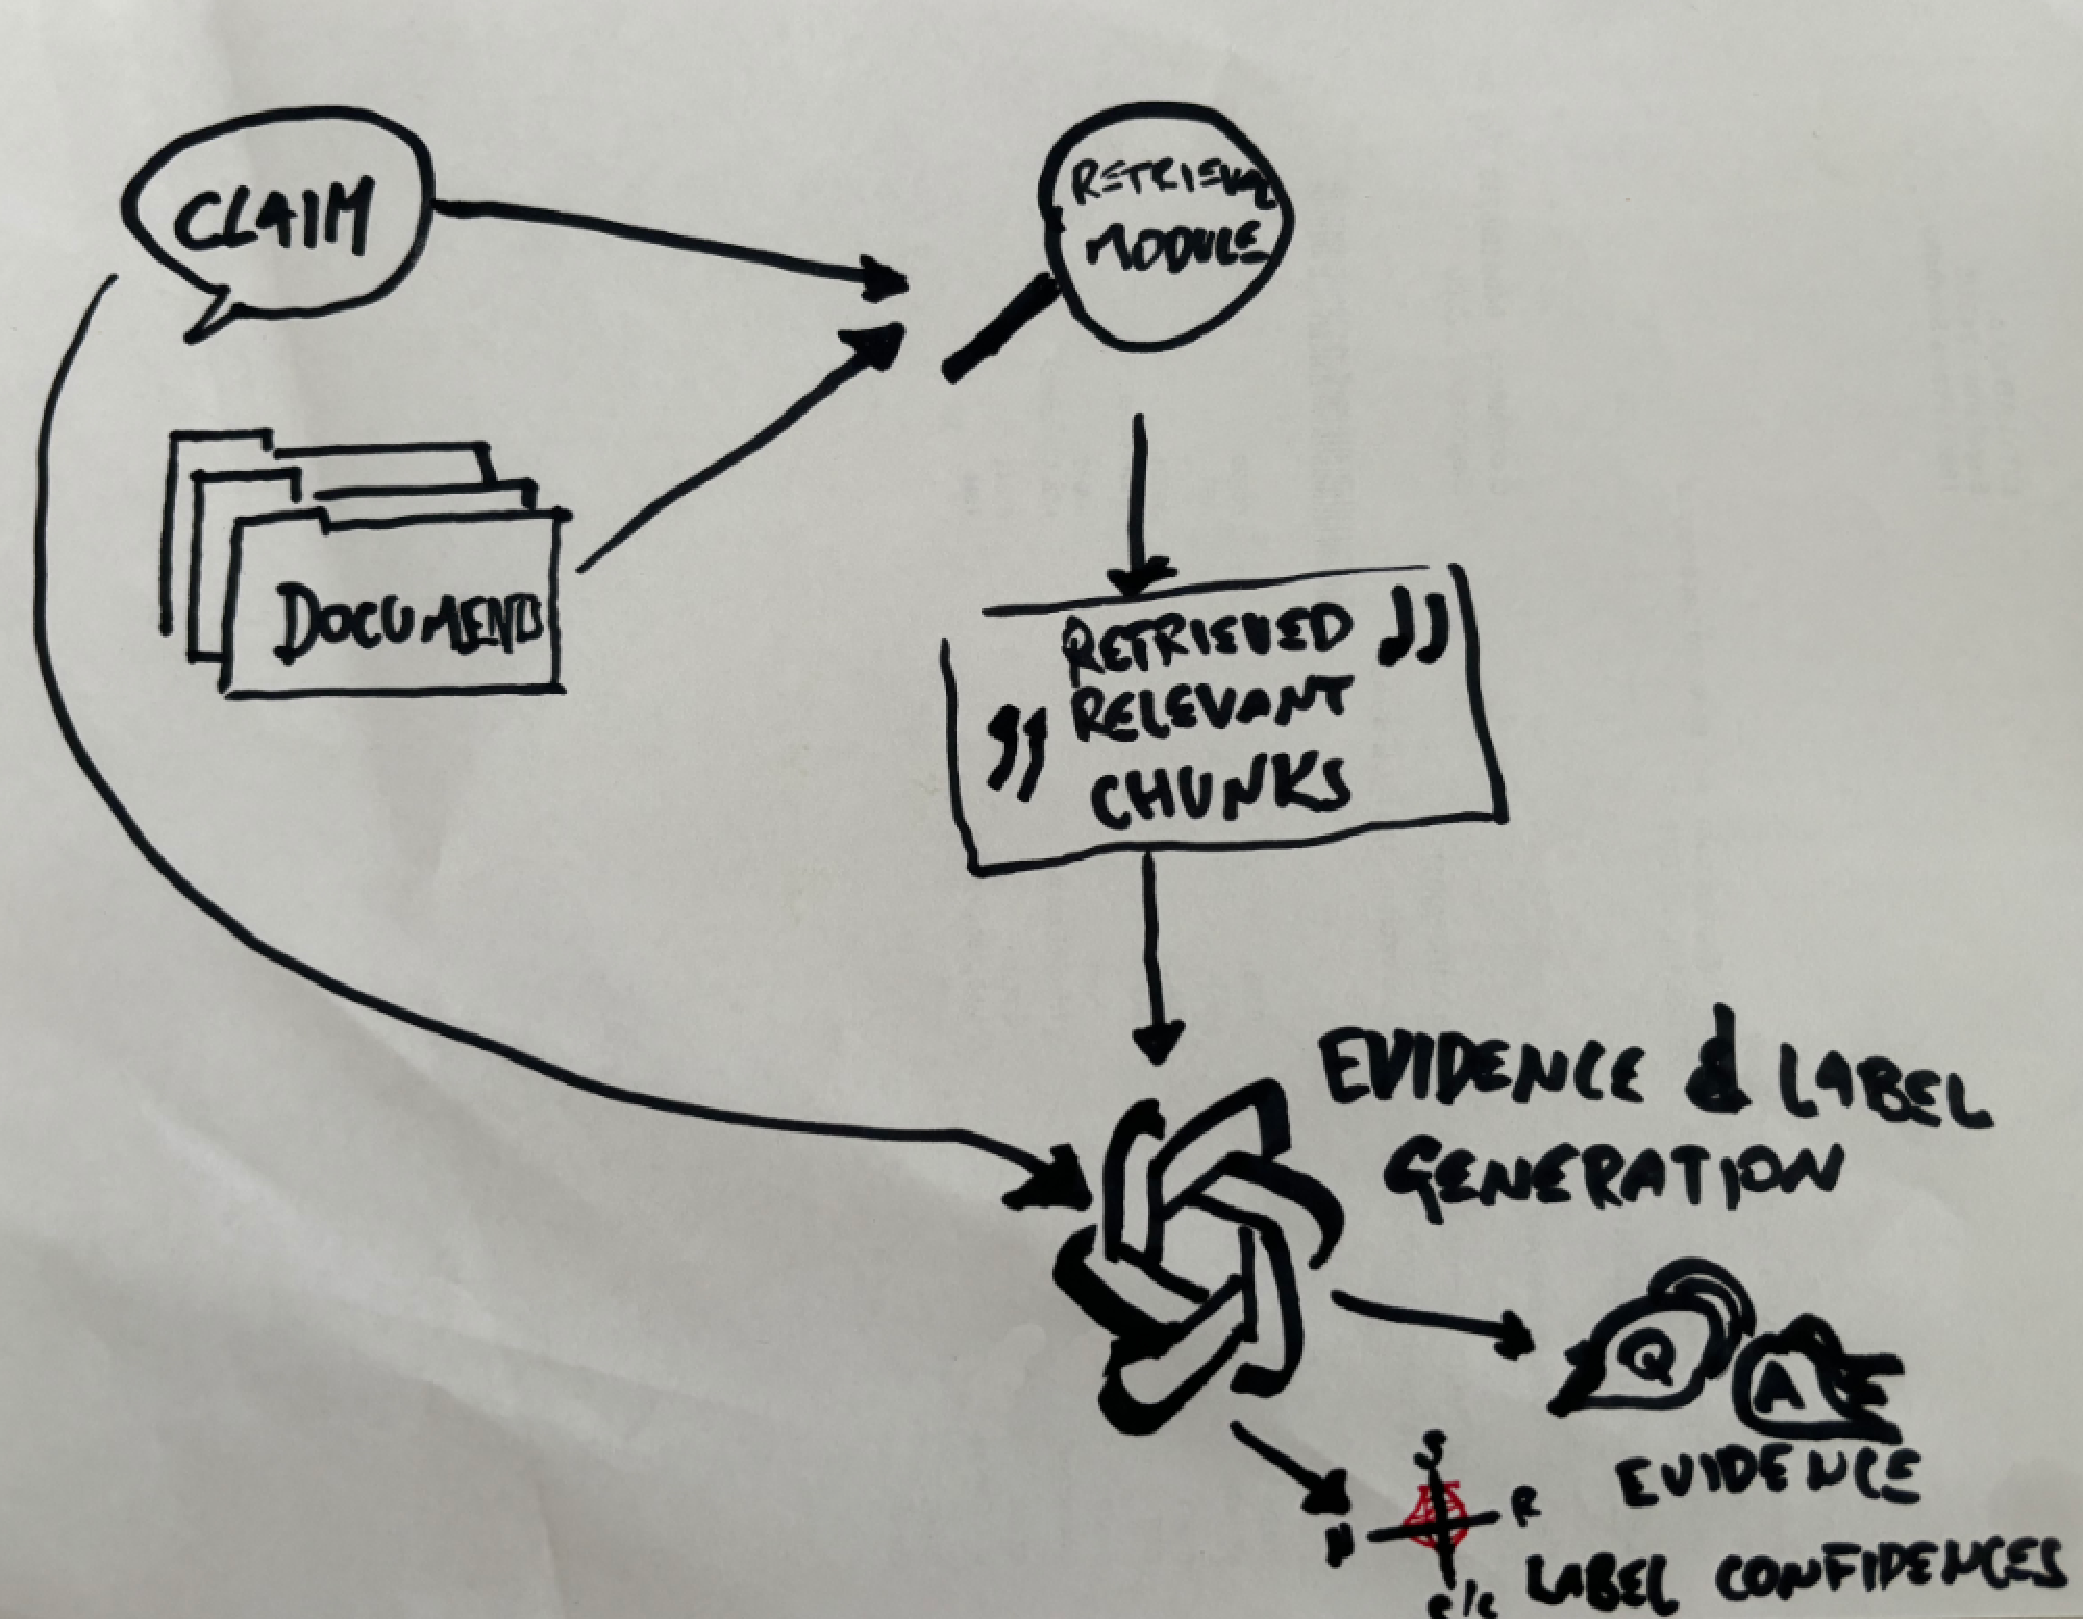
\includegraphics[width=0.47\textwidth]{figures/pipeline.pdf}
    \caption{Our pipeline}
    \label{fig:pipeline}
\end{figure}

\section{Related Work}
\label{sec:relwork}
\label{avscore}
\begin{enumerate}
    \item \textbf{\averitec{} shared task}~\cite{averitec2024} releases the dataset of real-world fact-checked claims, annotated with evidence available at the date the claim was made.
    
    It proposes the \textbf{\averitec{} Score} -- a method of unsupervised scoring of fact-checking pipeline against this dataset using Hungarian METEOR score (matching the evidence questions (Q) or the whole evidence (Q+A)), and then counting the proportion of claims with accurate label and sound evidence at the same time (using a threshold for Hu-METEOR such as 0.25) among all claims in the dataset, giving an estimate on \say{how often the whole fact-checking pipeline succeeds end to end}.

    The provided \textbf{baseline} is a pipeline of search query generation, API search (producing a knowledge store), sentence retrieval, Question-and-answer (QA) generation, QA reranking, QA-wise claim classification and label aggregation, achieving an overall \averitec{} score of 11\%.  
    \item \textbf{FEVER Shared Task}~\cite{thorne-etal-2018-fact}, a predecessor to the \averitec{} worked with a similar dataset engineered on top of the enclosed domain Wikipedic data rather than real-world fact-checks -- its top-ranking solutions used a simpler pipeline of Document Retrieval, Sentence Reranking and Natural Language Inference, improving its modules in a decoupled manner and scoring North of 60\% in a similarly computed FEVER score~\cite{thorne-etal-2018-fever} on this data.
    \item \textbf{Our previous research} on fact-checking pipelines~\cite{Ullrich2023,drchal2023pipelinedatasetgenerationautomated} using data similar to FEVER and \averitec{} shows significant superiority of fact-checking pipelines that \textbf{retrieve the whole documents} for the inference step, rather than retrieving out-of-context sentences.
    \item \textbf{Retrieval-Augmented Generation (RAG) for Knowledge-Intensive Tasks}~\cite{rag} takes this a step further, leveraging Large Language Model (LLM) for the task, providing it the whole text of retrieved documents (each a chunk of Wikipedia) and simply instructing it to predict the evidence and label on top of it, achieving results within 4.3\% from the FEVER state of the art by the time of its publication (December 2020) \textit{without} engineering a custom pipeline for the task.
\end{enumerate}


%!TEX ROOT=../emnlp2023.tex

\section{System Description}
\label{sec:system}
\todo{write}
Our syste

\subsection{Retrieval Module}
Mixedbread~\cite{li-li-2024-aoe,emb2024mxbai}, Faiss~\cite{douze2024faiss,johnson2019billion}

\subsubsection{Chunking}
Our initial experiments with the whole AVerITeC documents for the Document Retrieval step have revealed a significant weakness -- while the median document length (about 2000 characters) fits the input size of our embedding model with a generous margin, there is often a small number of documents with \textit{hundreds of thousands}§ characters, exceeding the 1024 input tokens with little to no coverage.

Upon further examination, these have more often than not, been PDF documents of legislature, documentation and transcription -- highly relevant sources real fact-checker would scroll through to find the relevant part to refer. 

This workflow has inspired our next approach -- to facilitate the retrieval of smaller articles as a whole and 

\subsubsection{Looking for diversity}
While the original~\cite{averitec2024} baseline retrieved articles based on different queries to promote variety among search result, our approach leverages the whole scope of given claim, without trying to divide its information, producing noise along the way.

To counterweight the relevancy-driven similarity search in the neighbourhood of a single \textit{query} embedding and its vulnerability to redundancy among search results, we perform reranking based on their Maximal Marginal Relevance (MMR)~\cite{carbonell-mmr}, a metric popular for the RAG task computed as
$$\lambda \cdot \mathrm{Sim}(D_i, Q) - (1-\lambda) \cdot \max_{D_j \in S} \mathrm{Sim}(D_i, D_j)$$

In our system, we set $\lambda=0.75$, $k=10$ and $k_{fetch} = 40$, already obtaining a result on par with a more complex system that would decompose the claim into subqueries and return results for each, using a fraction of its computational cost.

\subsection{Evidence Generation}
Rather than sampling evidence from retrieved text or QG+QA pipeline ran on the retrieved sentences, we argue that the modern LLMs offer the use of wider context, such as whole news articles.

\subsubsection{\texttt{JSON} Generation}
The current LLMs are trained very well for this, allows for very simple integration of LLM into pipeline

\subsubsection{Chain-of-thoughts Prompting}
While JSON dictionary should be order-invariant, we can actually exploit the order of outputs to make LLMS like GPT-4o output better results.

\subsubsection{Few-shot learning}




%!TEX ROOT=../emnlp2023.tex

\section{Classification Step}
In this section, we describe the classification component of our pipeline. First, we introduce chronologically the different approaches, the ensembles we tried, and their pros and cons. Then, we present evaluation results across different methods and various metrics. The goal of this step is to take the input claim and questions with answers provided by previous stages \todo{ref} and classify the claim into one of the four classes: \textit{Supported}, \textit{Refuted}, \textit{Not Enough Evidence}, or \textit{Conflicting Evidence/Cherrypicking} as defined by~\citealp{averitec2024}.

\subsection{Approaches}
\todo{Describe what was done +  why}

In the earliest stages of experimenting, we utilized the classifier from baseline provided by authors\footnote{https://huggingface.co/chenxwh/AVeriTeC}~\cite{averitec2024}. This classifier is based on BERT~\cite{devlin-etal-2019-bert} model and was further fine-tuned on the AVeriTeC dataset~\cite{averitec2024}. It takes one claim and one question with its answer as input. The output of this encoder model (class logits) is then further processed by several if-clauses to determine the final label. To the best of our knowledge, the complete classifier outputs \textit{Not Enough Evidence} every time when the model predicts the \textit{Not Enough Evidence} or some 4th label (here we are not sure how the model was exactly fine-tuned) for any of the (up to 10) question-anwer pairs. It predicts \textit{Supported} if there is no \textit{Not Enough Evidence} prediction and at least one \textit{Supported} prediction and no \textit{Refuted} prediction. Then it predicts \textit{Refuted} if there are no \textit{Not Enough Evidence} or \textit{Supported} predictions and at least one \textit{Refuted} prediction. Otherwise, it predicts \textit{Conflicting Evidence/Cherrypicking}. Despite considerable effort, we were unable to understand why and how was the model trained on four labels and also what is the exact background of this, at least from our point of view, ad-hoc post-processing logic.

We argue that the post-processing logic should be changed so that \textit{Not Enough Evidence} is predicted only if there is no other label to predicted. We think that for example if among the predictions for question-answer pairs there is one \textit{Not Enough Evidence} prediction and the rest are \textit{Supported} predictions, the final prediction should be \textit{Supported} and not \textit{Not Enough Evidence} as in the original logic. We did implemented this change (see listing~\ref{lst:post-processing}) and surprisingly it did not improve the results as the number of \textit{Not Enough Evidence} class has fallen significantly \todo{numbers}. Despite that, we still think that this change is more logical and should be used in the future.

\begin{figure}
    \begin{lstlisting}[language=Python]
if has_true and has_false:
  answer = 3
elif has_true and not has_false:
  answer = 0
elif not has_true and has_false:
  answer = 1
else:
 answer = 2 #otherwise NEI
        \end{lstlisting}
    \caption{Our proposed post-processing logic} 
    \label{lst:post-processing}       
\end{figure}

Moreover, we think that the model should be trained only on three labels because only three are used. We tried own fine-tuning of a newer encoder model DeBERTaV3~\cite{he2023debertav3improvingdebertausing} on only three labels and the results were better \todo{numbers}.

All of the results of our preliminary experimenting were however not satysfing and we decided to try more radically different approaches that are described in the following sections.

\subsubsection*{Concatenation and Four Classes Classificator}
\todo{better name}
\todo{describe, models, Concatenation, sep-concatenation, random order, four classes!, Mistral, DeBERTaV3, metion Transformers-HF}
Our first approach is to finetune a text classification model on all four classes directly. However, this means that as evidence, we must feed the model with all question-answer pairs at once to classify \textit{Conflicting Evidence/Cherrypicking} correctly. For that, we tried several options. First, we concatenated all of them using single blank space in the order they are provided in the dataset. This should work because we expect that annotators created the question-answer pairs usually in a specific order. The second option we tried is concatenation using a separator \texttt{[SEP]} token again in the original order. This option utilizes the model's knowledge about separator tokens and allows it to know exact question-answer borders. The last option we tried is to randomly select more orders of the question-answer pairs (all combinations computation is not feasible - up to $10!$ of combinations).

As models, we chose DeBERTaV3~\cite{he2023debertav3improvingdebertausing} in two variants: the original large one\footnote{https://huggingface.co/microsoft/deberta-v3-large} and one pre-finetuned on NLI tasks\footnote{https://huggingface.co/cross-encoder/nli-deberta-v3-large}, and also Mistral-7B-v0.3 model\footnote{https://huggingface.co/mistralai/Mistral-7B-v0.3} with a classification head (MistralForSequenceClassification) provided by the Huggingface Transformers library~\cite{wolf-etal-2020-transformers} that utilizes the last token. In the preliminary testing phase, the original DeBERTaV3 Large performed the best and was used in all other experimental settings.

From the approaches described above, we achieved the best results with the original order achieving 0.71 macro $F_1$ score. The separator model achieved a comparable 0.70 macro $F_1$ score, and the random order model performed worse with a 0.67 macro $F_1$ score. We provide our best DeBERTaV3 finetuned model publicly in a Huggingface repository\footnote{\todo{https://huggingface.co/ctu-aic/deberta-v3-large-AVeriTeC-nli}}.

\subsubsection*{LLM Classifiers}
\todo{describe - likert motivation, GPT4o, Claude 3?}
\todo{try "opensource" LLMs? - maybe own section in an Appendix?}

\subsubsection*{Ensembling}
\todo{describe ensembling - average, weighted average, stacking using logreg}

\subsubsection*{Conflicting Evidence/Cherrypicking Detection}
\todo{Binary deberta with custom loss function - weighted crossentropy loss}
\todo{Bryce's idea - tf-idf + randomforests?, future works-new paper (not exactly what we are doing now, but interesting)~\cite{jaradat2024contextawaredetectioncherrypickingnews}}


\subsection{Classification Evaluation}
\todo{table with comparative results + comments}

%!TEX ROOT=../emnlp2023.tex

\section{Results and analysis}
\label{sec:results}

We examine our pipeline results using two sets of metrics -- firstly, using the classification accuracy metrics over predicted labels without any ablation, that is obtaining the predicted labels using the predicted evidence generated on top the predicted retrieval results. While the retrieval module is fixed throughout this experiment (a full scheme described in section~\ref{retrieval}), various Evidence \& Label generators and classifiers are listed in Table~\ref{tab:nli} to give comparison on their performance on the same sources.
\begin{table}[H]
        \centering
    \setlength\tabcolsep{3pt} % default value: 6pt
    \resizebox{\columnwidth}{!}{%
    \begin{tabular}{lcccc}
        \toprule
        \textbf{Classifier} & \textbf{Acc} & \textbf{$F_1$} & \textbf{Prec.} & \textbf{{\footnotesize {Recall}}} \\
        \midrule
        GPT4o & \textbf{0.72} & 0.46 & 0.48 & 0.47 \\
        Claude 3.5 Sonnet & 0.64 & 0.49 & 0.50 & 0.52 \\
        DeBERTa & 0.63 & 0.39 & 0.40 & 0.41 \\
        DeBERTa - random@10 & 0.65 & 0.41 & 0.41 & 0.44 \\
        $0.5\cdot\mbox{DeBERTa}+0.5\cdot\mbox{GPT4o}$ & 0.70 & 0.43 & 0.41 & 0.45 \\
        $0.5\cdot\mbox{DeBERTa}+0.5\cdot\mbox{Claude}$ & 0.68 & 0.47 & 0.50 & 0.49 \\
        $0.3\cdot\mbox{DeBERTa}+0.7\cdot\mbox{GPT4o}$ & \textbf{0.72} & 0.45 & 0.45 & 0.46 \\
        $0.3\cdot\mbox{DeBERTa}+0.7\cdot\mbox{Claude}$ & 0.66 & \textbf{0.50} & \textbf{0.51} & \textbf{0.53} \\
        $0.1\cdot\mbox{DeBERTa}+0.9\cdot\mbox{GPT4o}$ & \textbf{0.72} & 0.39 & 0.46 & 0.43 \\
        $0.1\cdot\mbox{DeBERTa}+0.9\cdot\mbox{Claude}$ & 0.64 & 0.49 & 0.50 & 0.54 \\
        \midrule
        Llama 3.1 & 0.73 & 0.44 & 0.43 & 0.46 \\
        \bottomrule
    \end{tabular}
    }
    \caption{Evalution of the classifiers on the development set. $F_1$, Precision and Recall are computed as macro-averages. The random@10 suffix indicates that the classifier was tuned using 10 different random orders of QA pairs for each claim. GPT4o stands for the Likert classifier based on GPT-4o, Claude 3.5 Sonnet is the Likert classifier based on Claude 3.5 Sonnet, and DeBERTa is classifier based on DeBERTaV3 Large fine-tuned on \averitec{} gold evidence and labels.}
    \label{tab:nli}
\end{table}

\begin{table*}[h]
    \begin{table*}[h]
    \centering
    \begin{tabular}{l | c c c | c c c}
    \hline
    &\multicolumn{3}{c|}{\textbf{Dev Set Results}} & \multicolumn{3}{c}{\textbf{Test Set Results}}  \\
    \textbf{Pipeline Name} & \textbf{Q only} & \textbf{Q+A} & \textbf{AVeriTeC Score} & \textbf{Q only} & \textbf{Q+A} & \textbf{AVeriTeC Score} \\ \hline
    \textbf{mmr+gpt4o-dfewshot-atype}      & 0.46 & 0.29 & 0.42 & 0.46 & 0.32 & 0.50\\
    mmr+gpt4o-dfewshot-tiebrk-atype & 0.46 & 0.29 & 0.41 & 0.46 & 0.32 & 0.50\\
    \averitec{} baseline            & 0.24 & 0.19 & 0.09 & 0.24 & 0.20 & 0.11\\
    \hline
    submission\_dev\_gpt\_likert       & 0.45 & 0.27 & 0.39 \\
    dev\_subquery+gpt4o                & 0.45 & 0.28 & 0.40 \\
    
    dev\_mmr+gpt4o-dfewshot-mock       & 0.45 & 0.28 & 0.41 \\
    submission\_dev\_claude            & 0.43 & 0.28 & 0.35 \\
    submission\_dev\_claude\_likert   & 0.43 & 0.28 & 0.35 \\
    dev\_mmr+gpt4o-dfewshot-gpttiebreaking & 0.38 & 0.24 & 0.31 \\
    dev\_mmr+gpt4o-dfewshot            & 0.45 & 0.29 & 0.42 \\
    dev\_mmr+gpt4o-dfewshot-gpttie-10ev & 0.45 & 0.28 & 0.40 \\
    tuned weightavg gpt4o(?)+DeBERTa          & 0.45 & 0.27 & 0.39 \\
    tuned weightavg Claude(?)+DeBERTa          & 0.43 & 0.28 & 0.36 \\
    dev\_subquery+gpt4o-dfewshot       & 0.45 & 0.29 & 0.42 \\
    claude evidence - DeBERTa cls               & 0.43 & 0.28 & 0.33 \\
    gpt4o evidence - DeBERTa cls               & 0.45 & 0.28 & 0.36 \\
    dev\_mmr+gpt4o                     & 0.45 & 0.28 & 0.38 \\
    MMR+DynamicFewshot RAG            & & & & 0.46 & 0.31 & 0.49 \\
    AIC first test                     & & & & 0.45 & 0.30 & 0.47 \\
    mmr+claude-dynamic-fewshot          & & & & 0.42 & 0.30 & 0.46 \\
    
    \hline
    mmr+llama-dfewshot-tiebrk-atype & 0.46 & 0.27 & 0.36 & 0.47 & 0.29 & 0.42\\
    \bottomrule
    \end{tabular}
    \caption{Comparison of Pipeline Scores on Dev and Test Sets, AVeriTeC scores are @0.25}
    \label{tab:pipeline_scores}
\end{table*}
    
\end{table*}

\subsection{API costs}
During our experimentation July 2024, we have made around 9000 requests to OpenAI's \texttt{gpt-4o-2024-05-13} batch API, at a total cost of \$363.
This gives a mean cost estimate of \$0.04 per a single fact-check (or \$0.08 using the API without the batch discount) that can be further reduced using cheaper models, such as \texttt{gpt-4o-2024-08-06}.

We argue that such costs make our model suitable for further experiments alongside human fact-checkers whose time spent reading through each source and proposing each evidence by themselves would certainly come at a higher price.

Our successive experiments with LLaMa 3.1~\cite{meta2024llama31} show promising results as well, nearly achieving parity with GPT.
The use of open-source models such as LLaMa or Mistral allows running our pipeline on premise, without leaking data to a third party and billing anything else than the computational resources.
For further experiments, we are looking to integrate them into the attached Python library using VLLM~\cite{vllm}.

\subsection{Error analysis}
In this section, we provide the results of an explorative analysis of 20 randomly selected samples from the development set. We divide our description of the analysis into the pipeline and dataset errors.


\subsubsection{Pipeline errors}
Our pipeline tends to rely on unofficial (often newspaper) sources rather than official government sources, e.g., with a domain ending or containing \texttt{gov}. On the other hand, it seems that the annotators prefer those sources. This could be remedied by implementing a different source selection strategy, preferring those official sources. For an example, see Listing~\ref{lst:gov_error}.

Another thing that could be recognised as an error is that our pipeline usually generates all ten allowed questions (upper bound given by the task~\cite{averitec2024}). The analysis of the samples shows that the last questions are often unrelated or redundant to the claim and do not contribute directly to better veracity evaluation. However, since the classification step of our pipeline is not dependent on the number of question-answer pairs, this is not a critical error. Moreover, when the pipeline is evaluated using the \averitec{} dataset evaluation, it slightly helps with the perfect matching step using the Hungarian algorithm. Listing~\ref{lst:unrelated_questions} shows an example of a datapoint with some unrelated questions.

When the pipeline generates extractive answers, it sometimes happens that the answer is not precisely extracted from the source text but slightly modified. An example of this error can be seen in Listing~\ref{lst:extractive_error}. This error is not critical, but it could be improved in future works, e.g. using post-processing via string matching.

Individual errors were also caused by the fact that we do not use the claim date in our pipeline and because our pipeline cannot analyse PDFs with tables properly. The last erroneous behaviour we have noticed is that the majority of questions and answers are often generated from a single source. This should not be viewed as an error, but by introducing diversity into the sources, the pipeline would be more reliable when deployed in real-world scenarios.

\subsubsection{Dataset errors}
During the error analysis of our pipeline, we also found some errors in the \averitec{} dataset that we would like to mention. In some cases, there is a leakage of PolitiFact fact-checking articles where the claim is already fact-checked. This leads to a situation where our pipeline gives a correct verdict using the leaked evidence. However, annotators gave a different label (often Not Enough Evidence). 

Another issue we have noticed is the inconsistency in the questions and answers given by annotators. Sometimes, they are long, including non-relevant information, but sometimes, they are at the correct length. The questions are often too general, or the annotators seem to use outside knowledge. This inconsistency in the dataset leads to a decreased performance of any models evaluated on this dataset.

\subsubsection{Summary}
Despite the abovementioned errors, the explorative analysis revealed that our pipeline consistently gives reasonable questions and answers for the claims. Most misclassified samples in those 20 data points were due to dataset errors.


%%!TEX ROOT=../emnlp2023.tex

\section{Python Library}
\label{sec:software}
\todo{write}
To facilitate further experimentation with our pipeline and the reusal of all the tools prompts and software, we have published our code as ready-to-use python library.

The retrieval, evidence generation and veracity inference steps are  \texttt{EvidenceGenerator}
%!TEX ROOT=../emnlp2023.tex

\section{Conclusion}
\label{sec:conclusion}
In this paper, we describe the use and development of a RAG pipeline over real world claims and data scraped from the web for the \averitec{} shared task.
Its main advantage are its simplicity, consisting of just two decoupled modules -- Retriever and an Evidence~\& Label Generator -- and leveraging the trainable parameters of a LLM rather than on complex pipeline engineering.
The LLMs capabilities may further improve in future, making the upgrades of our system trivial.

In section~\ref{sec:system}, we describe the process of adding features to both modules well in an iterative fashion, describing real problems we have encountered and the justifications of their solution, hoping to share our experience on how to make such systems robust and scoring well.
We publish our failed approaches in section~\ref{sec:failed} and the metrics we observed to benchmark our systems in section~\ref{sec:results}. 
We release our Python codebase to facilitate further research and applications of our system, either as a baseline for future research, or for experimenting alongside human fact-checkers.

\subsection{Future works}
\begin{enumerate}
    \item Integrating a search API for use in the wild 
    \item Re-examine the Likert-scale rating (section~\ref{likert}) to establish a more appropriate and fine-grained means of tokenizing the label probabilities
    \item Generating evidence in the form of declarative sentences rather than Question-Answer pairs should be explored to see if it leads for better or worse fact-checking performance
    \item RAG-tuned LLMs such as those introduced in~\cite{menick2022teachinglanguagemodelssupport} could be explored to see if they offer a more reliable source citing
\end{enumerate}
%%%%%%%%%%%%%%%%%%%%%%%%%%%%%%%%%%%%

\section*{Limitations}
\todo{Je to testovany jen v EN, neni to skutecny factchecker ale jen poc studie jeho proveditelnosti a kvantifikace toho jak moc to uz dnes jde 2. diskriminuje to pristupem k velkymu compute, bud posles velky firme data nebo nakoupis drahy compute. 3. ma to uhlikovou stopu jak traktor. Neprosli jsme ta data. - TM: Možná spolehlivost? Můžeme se spolehnout že nebude halucinovat, používat jiné zdroje apod?}

\section*{Ethics Statement}
\todo{tohle bude potreba: 1. neni to skutecny plugnplay factchecker, ale studie jeho budouci proveditelnosti 2. tim ze to bylo tuneny na uspech nad \averitec{}  sadou tak to odrazi zaujeti jeho anotatoru (todo citace).}

\todo{emlp ethics faq: https://2021.emnlp.org/call-for-papers/ethics-faq - sections ...if my paper involves an NLP application?, ... if my paper reports on experiments that involve lots of compute time/power?}

\section*{Acknowledgements}
We would like to thank Bryce Aaron from UNC for exploring the problems of search query generation and pinpointing claims of underrepresented labels using numerical methods that did not make it into our final pipeline but gave us a frame for comparison. 

This research was co-financed with state support from the Technology Agency of the Czech Republic and the Ministry of Industry and Trade of the Czech Republic under the TREND Programme, project FW10010200.
The access to the computational infrastructure of the OP VVV funded project CZ.02.1.01/0.0/0.0/16\_019/0000765 ``Research Center for Informatics'' is also gratefully acknowledged.
We would like to thank to OpenAI for providing free credit for their paid API via Researcher Access Program\footnote{https://openai.com/form/researcher-access-program/}.



% Entries for the entire Anthology, followed by custom entries
\bibliography{anthology,custom}
\bibliographystyle{acl_natbib}

\appendix

%!TEX ROOT=../emnlp2023.tex


\lstset{
    language={},
    basicstyle=\ttfamily\footnotesize\linespread{0.9}, % Smaller font with less spacing
    keywordstyle=\color{blue}\bfseries,
    commentstyle=\color{green!50!black}\itshape,
    stringstyle=\color{orange},
    numberstyle=\tiny\color{gray},
    numbers=left, % Line numbers on the left
    stepnumber=1, % Line numbers for every line
    numbersep=5pt, % Space between line numbers and code
    tabsize=4, % Size of tabs
    showstringspaces=false, % Don't show spaces in strings
    breaklines=true, % Line wrapping
    breakatwhitespace=true,
    frame=lines, % Add a frame around the code
    captionpos=b, % Caption at the 
    breakindent=1em,
}
\begin{figure*}
    \section{System Prompt}
    \label{System Prompt}
    \begin{lstlisting}[breaklines=true, language={}, frame=single, caption={System prompt for the LLMs, \averitec{} claim is to be entered into the user prompt. Three dots represent omitted repeating parts of the prompt.}, label={lst:llm_system_prompt}]
You are a professional fact checker, formulate up to 10 questions that cover all the facts needed to validate whether the factual statement (in User message) is true, false, uncertain or a matter of opinion. Each question has one of four answer types: Boolean, Extractive, Abstractive and Unanswerable using the provided sources.
After formulating Your questions and their answers using the provided sources, You evaluate the possible veracity verdicts (Supported claim, Refuted claim, Not enough evidence, or Conflicting evidence/Cherrypicking) given your claim and evidence on a Likert scale (1 - Strongly disagree, 2 - Disagree, 3 - Neutral, 4 - Agree, 5 - Strongly agree). Ultimately, you note the single likeliest veracity verdict according to your best knowledge.
The facts must be coming from these sources, please refer them using assigned IDs:
---
## Source ID: 1 [url]
[context before]
[page content]
[context after]
...

---
## Output formatting
Please, you MUST only print the output in the following output format:
```json
{
 "questions":
     [
         {"question": "<Your first question>", "answer": "<The answer to the Your first question>", "source": "<Single numeric source ID backing the answer for Your first question>", "answer_type":"<The type of first answer>"},
         {"question": "<Your second question>", "answer": "<The answer to the Your second question>", "source": "<Single numeric Source ID backing the answer for Your second question>", "answer_type":"<The type of second answer>"}
     ],
 "claim_veracity": {
     "Supported": "<Likert-scale rating of how much You agree with the 'Supported' veracity classification>",
     "Refuted": "<Likert-scale rating of how much You agree with the 'Refuted' veracity classification>",
     "Not Enough Evidence": "<Likert-scale rating of how much You agree with the 'Not Enough Evidence' veracity classification>",
     "Conflicting Evidence/Cherrypicking": "<Likert-scale rating of how much You agree with the 'Conflicting Evidence/Cherrypicking' veracity classification>"
 },
 "veracity_verdict": "<The suggested veracity classification for the claim>"
}
```
---
## Few-shot learning
You have access to the following few-shot learning examples for questions and answers.:

### Question examples for claim "{example["claim"]}" (verdict {example["gold_label"]})
"question": "{question}", "answer": "{answer}", "answer_type": "{answer_type}"
...
    \end{lstlisting}
\end{figure*}
%%!TEX ROOT=../emnlp2023.tex

\section{Open-Source LLMs}
\label{appendix_sec:opensource_llms}

\end{document}
